\chapter{Description of the Work}
\label{chapter:description}
% Spieghiamo cose abbiamo fatto prima di fare il lavoro vero e proprio, comprendendo eventuali problemi incontrati
\section{Preliminary Setup and Experimentation}

The machine used for testing and development for this work has the following main characteristics:

\begin{itemize}[noitemsep]
	\item Processor: Intel i7 6700HQ
	\item RAM: 16 GB
	\item OS: Ubuntu 16.04
\end{itemize}

Before starting our work, we followed a basic guide \cite{tutorial} for the Zynq Zedboard platform. These tutorials proved to be very useful to the team in order to grasp the basics of the platform. After setting up the environment, we built the first application, named \texttt{HelloWorld}, that simply sends its name to the UART interface.

% Spieghiamo come far si che il sistema si accorga della board su un sistema Linux
\subsection{Linux Configuration}

While on Windows machines the detection on the board may be automatic due to Windows Update, for a Linux system two packages are required. They are the Adept Runtime and Adept Utilities packages, that can be obtained from the Digilent website. If these two packages are not installed on the machine, then both Vivado and the SDK will not recognize the board when connected, effectively rendering impossible any kind of configuration.

% Spieghiamo come abbiamo implementato la funzionalità per misurare il tempo trascorso
\subsection{Timer Experimentation}
The first thing that we tried was a simple measure of the execution time of the \texttt{HelloWorld} application. We followed the tutorial released by AVNET modifying the \texttt{C++} code. We included the \texttt{XTime\_l.h} library. Doing this we can get the Global Timer Counter Register value in order to compute the time elapsed to print "Hello world" using the UART connection to the PC. The new code is in figure \ref{fig:helloworldtimer}.

\begin{figure}[htbp]
	\centering
	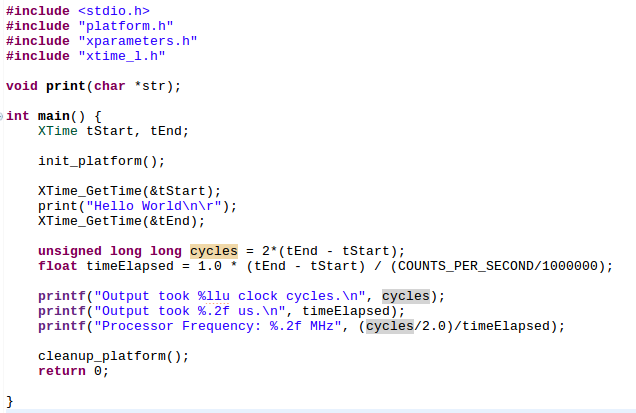
\includegraphics[width=0.85\textwidth]{timerHelloWorld}
	\caption{Time evaluation for the \texttt{HelloWorld} application}
	\label{fig:helloworldtimer}
	
	\bigskip
	\noindent
	\begin{flushleft}
		The ARM core is processing at 333 MHz, that is the configured frequency, as shown in figure \ref{fig:helloworldtimeroutput}.
	\end{flushleft}
	\bigskip
	
	\centering
	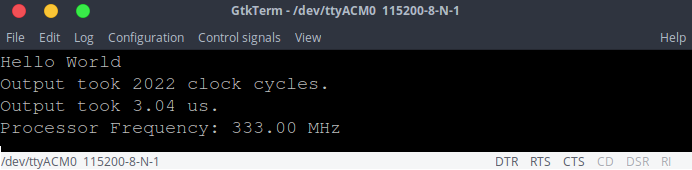
\includegraphics[width=0.85\textwidth]{GTKHelloWorldTimerOutput}
	\caption{UART output on GTKTerm (on PC)}
	\label{fig:helloworldtimeroutput}
\end{figure}

\section{Context of the Work}
% "One general scheme of your work that allows to understand where your work fits"
Our work is strictly related to the CC4CS project\cite{cc4cs_git} (acronym for \textit{Clock Cycles for C Statement}). CC4CS is the ratio between the number of clock cycles required by the processor to run an application and the number of executed C statements. A framework that helps to calculate this metric has been developed:

\[
\text{CC4CS} = \frac{\text{Number of Clock Cycles}}{\text{Executed C Statements}}
\]

This framework aims to help engineers estimate the execution time of their applications, described in C, on FPGA. This would give the designer a way to work with estimations before choosing the final platform.

\subsection{Tested Algorithms}
\label{tested-algo}

The algorithms used to test the framework are the following.

\begin{itemize}[noitemsep]
	\item Selection Sort
	\item Bubble Sort
	\item Merge Sort
	\item Quick Sort
	\item Insertion Sort
	\item Greatest Common Divisor
	\item Floyd-Warshall's Algorithm
	\item Bellman-Ford's Algorithm
	\item Banker's Algorithm

\end{itemize}

A detailed explanation of the algorithms' characteristics is in appendix \ref{app:algoritmi}.

Time and space estimations for an initial VHDL/Verilog implementation of these algorithms are available in section \ref{sec:spacetime_estimations}. These estimations have been performed using these parameters:
\begin{itemize}[noitemsep]
	\item \textbf{Sorting Algorithms}: input array with dimension 10, with type \textbf{float} or \textbf{long}
	\item \textbf{GCD Algorithm}: testbench made using arbitrary \textbf{integer} numbers
	\item \textbf{Graph Algorithms}: input (adjacency) matrix with dimension $10\times10$
	\item \textbf{Banker's Algorithm}: testbench made using 4 processes and 3 resources

\end{itemize}